\documentclass{article}
\usepackage{tikz}
\usepackage{hyperref}
\usepackage[a4paper]{geometry}
\usepackage{fancyhdr}
\pagestyle{fancy}
\lhead{Mechanische Wellen}
\rhead{September 2025}
\begin{document}
\section{Mechanische Wellen} 
Eine mechanische Welle ist eine örtliche und zeitliche periodische Veränderung einer physikalischen Größe. Dem \emph{Resonanzprinzip} nach wird die Energie eines \emph{Erregers} über die Kopplung mit einem benachbarten schwingungsfähigen System auf dieses übertragen.
 
Eine mechanische Welle kann sich sozusagen als eine \hyperref[Mechanische Schwingungen]{mechanische Schwingung} vorgestellt werden, welche sich aber darüberhinaus örtlich weiterverbreitet.
\begin{center} 
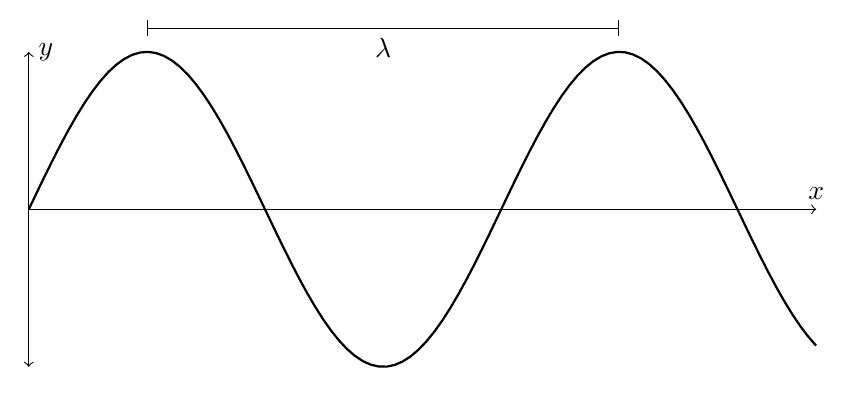
\begin{tikzpicture}
 \draw[->] (0, 0) -- (10, 0) node[above] {$x$};
 \draw[<->] (0, -2) -- (0, 2) node[right] {$y$};
 \draw[thick, domain=0:10, samples=100] 
            plot (\x, {2*sin(\x*360 / 6)});
 
 \draw[|-|] ({6/4}, 2.3) -- ({6*1.25}, 2.3) node[midway, below] {$\lambda$};
\end{tikzpicture} 
\end{center}
 
\subsection{Größen} 
Eine Welle hat eine \emph{Wellenlänge} $\lambda$, welche beschreibt, wie weit eine Welle sich örtlich während einer Periodendauer. Wird die Welle als Sinusfunktion dargestellt, ist $\lambda$ eine Periode. Daraus folgt auch, dass Wellen eine \emph{Ausbreitungsgeschwindigkeit} $c$ haben
\[
 c = \frac{\lambda}{T} = \lambda \cdot f 
\]
Mit der obigen Darstellung ist es klar, dass die Welle in der Zeit $T$ sich um eine Distanz $\lambda$ ausgebreitet hat. In Analogie zu $v=s/t$ ist die obige Formel also offensichtlich. 
 
Die Sinusfunktion kann um die Phase $\varphi$ verschoben sein. 
 
\subsection{Schwingungsrichtungen} 
Es wird bei mechanischen Wellen in zwei Schwingungsrichtungen unterschieden
\begin{description}
 \item[Transversalwellen] Teilchen schwingen senkrecht zur Ausbreitungsrichtung
 \item[Longitudinalwellen] Teilchen schwingen in Ausbreitungsrichtung, z.\,B. Schallwellen
\end{description} 
\end{document}